\def\currentRootFolder{chapter/sensitivityStudyWithPreliminaryKatrinElossModel/statisticalPrerequisites}
\def\currentFigureFolder{\currentRootFolder/fig}
\newcommand{\elecIndex}{\mathrm{e}}

\newcommand{\Bsource}{B^j_\mathrm{S}}
\newcommand{\BsourceAvg}{B_\mathrm{S}}
\newcommand{\zSource}{z_\mathrm{S}}
\newcommand{\thetaSource}{\theta_\mathrm{S}}
\newcommand{\thetaSourceAvg}{\theta_\mathrm{S}}
\newcommand{\Esource}{E_\mathrm{S}}
\newcommand{\Usource}{U^j_\mathrm{S}}
\newcommand{\gammaSource}{\gamma_\mathrm{S}}


\newcommand{\Bps}{B_\mathrm{PS2}}
\newcommand{\Bana}{B_\mathrm{A}}
\newcommand{\Bpinch}{B_\mathrm{P}}
\newcommand{\Bmax}{B_\mathrm{max}}
\newcommand{\Bmin}{B_\mathrm{min}}

\newcommand{\thetaMax}{\theta_\mathrm{max}}
\newcommand{\Esur}{E_\mathrm{sur}}
\newcommand{\detEff}{\epsilon_\mathrm{det}}
\newcommand{\macefilterwidth}{\Delta \mathcal{E}^j(\thetaS^j)}

\newcommand{\EtransPure}{E^j_\mathrm{tr}}
\newcommand{\Etrans}{\EtransPure(qU,\Esource,\thetaSource)}
\newcommand{\thetaTransPure}{\theta^j_\mathrm{tr}}
\newcommand{\thetaTrans}{\thetaTransPure(\Esource,qU)}

\newcommand{\As}{A_\mathrm{S}}
\newcommand{\Rbg}{R_\mathrm{bg}}


\newacronym{standardmodel}{SM}{Standard Model of Particle Physics}
\newacronym{lep}{LEP}{Large Electron Positron Collider}
\newacronym{ssm}{SSM}{standard solar model}

\section{Statistical Prerequisites}
\label{sec:katrinElossStatistics}
This section develops the statistical tools used in the scope of this thesis in order to evaluate the impact of the KATRIN model on KATRIN's sensitivity to the neutrino mass. The methods are described in a general manner (and could be applied to study model uncertainties in general) and then related to the KATRIN model. Section~\ref{sec:katrinElossStatisticsCombMeasurements} presents a concept for the combination of a neutrino mass and a commissioning measurement in parameter inference. Section~\ref{sec:katrinElossStatisticsProfileLikelihood} introduces the profile-likelihood method for the treatment of nuisance parameters. Section~\ref{sec:katrinElossStatisticsAsimov} relates ensemble testing and Asimov data sets.

\subsection{Combination of Commissioning and Neutrino Mass Measurements}
\label{sec:katrinElossStatisticsCombMeasurements}
If two measurements share a set of parameters $\paramVecShared$, but have additionally an individual set of parameters $\paramVec_1$ and $\paramVec_2$ and different sets of observations a combined likelihood is given by the product of the single likelihoods $L_1$ and $L_2$~\cite{ReviewOfParticlePhysics}
\newcommand{\paramVecSOne}{\paramVec_\mathrm{s,1}}
\newcommand{\paramVecSTwo}{\paramVec_\mathrm{s,2}}
\begin{align}
-2\ln L(\paramVecShared, \paramVec_1, \paramVec_2) &=  
-2\ln L_1(\paramVecShared, \paramVec_1)
-2\ln L_2(\paramVecShared, \paramVec_2)
\nonumber \\
&\equiv
-2\ln L_1(\paramVecSOne)
-2\ln L_2(\paramVecSTwo)
\fullstop
\end{align}
where, for ease of notation, the combined parameter vectors $\paramVec_\mathrm{s,1}\equiv(\paramVec_\mathrm{s},\paramVec_1)$ and 
$\paramVec_\mathrm{s,2}\equiv(\paramVec_\mathrm{s},\paramVec_2)$ are introduced. The first measurement could be sensitive to the neutrino mass whereas the second measurement could have been a calibration or commissioning measurement and be sensitive to parameters of the response function (see equation~\ref{eq:intSpecModelResponse}). Combining both likelihoods would incorporate the uncertainties on the parameters of the response function in the neutrino mass determination. 

For practicality, in this thesis, an approximation is applied: The calibration measurement is seen as evaluated independently and one obtains estimates $\hat{\paramVec}_\mathrm{s,2}$, and an estimated covariance matrix $\hat{V}_\mathrm{s,2}$. These can in turn be used to approximate the likelihood $L_2$. A choice that stands to reason for the approximation of $L_2$ is a multivariate normal distribution $\mathcal{N}$. For the purpose of parameter inference through the maximum likelihood method $-2\ln L_2$ needs only to be accurately approximated within the contour, that is needed to extract uncertainty intervals. The choice of a multivariate normal distribution corresponds a symmetric approximation of $-\ln L_2$ around its minimum by a second order function. The combined likelihood then reads
\begin{equation}
\begin{split}
\label{eq:katrinElossStatisticsPullTerm}
-2\ln L(\paramVecShared, \paramVec_1, \paramVec_2) &\approx
\chi^2(\paramVecSOne) 
-2\ln \mathcal{N}(\paramVecSTwo, \hat{\paramVec}_\mathrm{s,2}, \hat{V}_\mathrm{s,2}^{-1}) +
\mathrm{ constants}\\ &=
\underbrace{
	\chi^2(\paramVecSOne)
	\vphantom{(\paramVecSTwo - \hat{\paramVec}_\mathrm{s,2})^{\mathsf{T}}}
}_{(1)}
+
\underbrace{
	(\paramVecShared - \hat{\paramVec}_\mathrm{s,2})^{\mathsf{T}}
	\hat{V}_\mathrm{s,2}^{-1}
	(\paramVecShared - \hat{\paramVec}_\mathrm{s,2})
}_{(2)} +\; 
\mathrm{ constants}
\end{split}
\end{equation}
Here, $(1)$ is the chi-square likelihood for a KATRIN neutrino mass measurement (see equation~\ref{eq:statMethodsKatrinChi2}). And $(2)$ resembles the negative log likelihood of the calibration measurement approximated by a multivariate normal distribution. Terms having a form like $(2)$ are also sometimes called ``pull terms'' because in the minimization of the likelihood they ``pull'' the parameters $\paramVecShared$ towards the corresponding values in $\hat{\paramVec}_\mathrm{s,2}$.

The chi-square term $(1)$ is a sum of $n$ standard normal distributed random variables. Hence, as discussed in section~\ref{sec:statMethodsKATRINLikelihood}, a likelihood only composed of the chi-square term $(1)$ offers a goodness-of-fit criteria via the the Pearson chi-square statistic. Whether the same criteria can be applied to the combined likelihood has to be investigated individually from case to case.

\paragraph{Application to the KATRIN Energy Loss Model}
With regard to the study presented in this chapter, the following identification can be made. $\paramVec_1$ comprises the parameter of a nominal four-parameter KATRIN neutrino mass fit (see section~\ref{sec:statMethodsStandardFit}). Furthermore, the commissioning/calibration measurement can be identified with the measurement of the KATRIN energy loss model $\hat{\paramVec}_\mathrm{s}=\hat{\nuisanceParamVec}_\mathrm{eloss}$, $\hat{\paramVec}_2=\hat{\nuisanceParamVec}_\mathrm{eloss+}$ (see equations~\ref{eq:katrinElossElossModelParams}~and~\ref{eq:katrinElossElossModelExtendedParams}) and the corresponding estimator for the covariance matrix $\hat{V}_\mathrm{s,2}=\hat{V}_\mathrm{eloss,eloss+}$. The numerical values for the later three can be found in the form of the means, the standard deviations and the correlation matrix in appendix~\ref{sec:appendixKatrinElossElossModelParams}.

\paragraph{Implementation in the KaFit Software Framework}
The KaFit software module (see section~\ref{sec:statMethodsKaFitSSC}) had allowed to use one-dimensional Gaussian ``pull terms'' (term $(2)$ in equation~\ref{eq:katrinElossStatisticsPullTerm}). In the scope of this thesis the software was extended to allow for arbitrary dimensions with corresponding correlations by using a multivariate normal distribution. Albeit not of particular interest in this chapter, for completeness, the following shall be mentioned: By comparing equations~\eqref{eq:statMethodsPosterior} and~\eqref{eq:katrinElossStatisticsPullTerm} it becomes apparent that such ``pull terms'' take the same mathematical form as Bayesian priors. For that reason further term forms apart from the multivariate normal distribution were implemented in order to be used in a Bayesian analysis. For a documentation of the software features see appendix~\ref{sec:appendixKatrinElossStatisticsLikelihoodExtKaFitConfig}.

\subsection{Nuisance Parameters and the Profile-Likelihood Method}
\label{sec:katrinElossStatisticsProfileLikelihood}
\begin{figure}[t]
	\centering
	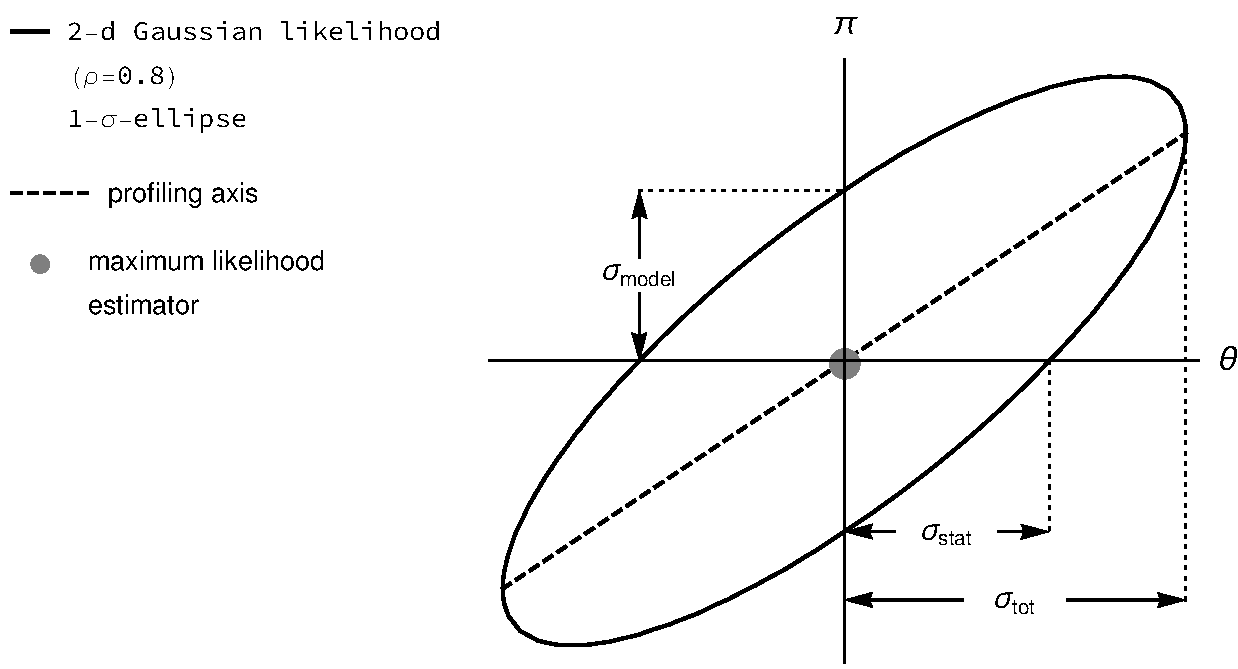
\includegraphics[width=\textwidth]{\currentFigureFolder/profileLikelihood.pdf}
	\xcaption{Illustration of the profile-likelihood method}{Illustration of the profile-likelihood method.}{The graph illustrates the extraction of a confidence interval from the likelihood in a two-dimensional scenario, where there is only one nuisance parameter $\pi$ and one parameter of interest $\theta$. The graph is a contour plot of an exemplary two-dimensional likelihood of Gaussian shape with a correlation between $\pi$ and $\theta$ of $\rho=0.8$. The contour encloses a 1-$\sigma$-confidence region as per equation~\eqref{eq:statMethodsConfidenceContour}. Its width in the dimension of $\pi$ is indicated as ``model''-uncertainty with reference to an uncertainty stemming from a model established by a commissioning measurement as described in section~\ref{sec:katrinElossStatisticsCombMeasurements}. The width in the dimension of $\theta$ stems from the statistical uncertainty. The dashed line contains the points $\left(\theta, \hat{\hat{\pi}}(\theta)\right)$ as per equation~\eqref{eq:katrinElossStatisticsProfileLikelihoodRatio}. It always intersects the contour at the point furthest right and left in the dimension of $\theta$ independently of $\rho$, $\sigma_\mathrm{stat}$ and $\sigma_\mathrm{model}$. The point of intersection determines $\sigma_\mathrm{tot}$. For example MINOS of the ROOT software framework is an algorithm that numerically tries to find the intersection of the dashed line and the contour. Under the conditions stated in the main text, the interval of width $2\cdot\sigma_\mathrm{tot}$ on the $\theta$ axis around the maximum likelihood estimator is per construction a confidence \mbox{interval (\SI{68}{\percent} C.L.)} for the true value of $\theta$. A feature that can intuitively be deduced from the graph is the following: No matter how much $\sigma_\mathrm{model}$ is reduced, the total uncertainty $\sigma_\mathrm{tot}$ can never shrink below $\sigma_\mathrm{stat}$. Likewise, whether a longer measurement, that decreases $\sigma_\mathrm{stat}$, can improve $\sigma_\mathrm{tot}$ depends on $\sigma_\mathrm{model}$ and the correlation $\rho$.}
	\label{fig:katrinElossStatisticsProfileLikelihood}
\end{figure}
Apart from the  parameters of interest $\paramVec$ (usually the squared neutrino mass), the KATRIN likelihood depends on further nuisance parameters $\nuisanceParamVec$. The dimensionality may pose computational difficulties when deriving a confidence region for the combined parameter set. Furthermore, as indicated by the naming conventions, the dimensions of the nuisance parameters in the confidence region are not of interest. Hence, in order to construct a confidence interval with just one dimension, a test statistic, similar to the one in equation~\ref{eq:statMethodsLikelihoodRatio}, but solely depending on the parameters of interest, has to be found. The following paragraph outlines, how a corresponding test statistic can be constructed using the profile-likelihood method.

First, the profile likelihood is defined. It only depends on the parameters of interest $\paramVec$ and is independent of the nuisance parameters $\nuisanceParamVec$. Its values correspond the likelihood values evaluated at $\paramVec$ in the dimensions of the parameters of interest and maximized in the dimensions of the nuisance parameters~\cite{ReviewOfParticlePhysics}
\begin{equation}
\label{eq:katrinElossStatisticsProfileLikelihood}
\profLikelihood(\paramVec) = 
L(\paramVec, \hat{\hat{\nuisanceParamVec}}(\paramVec))
\comma
\end{equation}
where the double-hat indicates the maximization respectively the profiling. Also, the profile likelihood ratio can be defined~\cite{ReviewOfParticlePhysics}
\begin{equation}
\label{eq:katrinElossStatisticsProfileLikelihoodRatio}
\lambda_\mathrm{p}(\paramVec) = 
\frac{\profLikelihood(\paramVec)}{\profLikelihood(\hat{\paramVec})}
\fullstop
\end{equation}
According to Wilks’ theorem~\cite{wilks1938}, the distribution of $-2\ln\lambda_\mathrm{p}(\hat{\paramVec})$, where $\hat{\paramVec}$ is the \gls{mle} (see section~\ref{sec:statMethodsMLE}), approaches a chi-square distribution in the limit of a large data sample, independently of the values of the nuisance parameters $\nuisanceParamVec$~\cite{ReviewOfParticlePhysics}. Hence, the profile likelihood ratio offers a test statistic, from which a confidence interval for the parameters of interest can be derived. However, it should be noted that whether the limit of a large sample is given has to be investigated individually from case to case.

Figure~\ref{fig:katrinElossStatisticsProfileLikelihood} illustrates the profile-likelihood method for the case where $\paramVec$ and $\nuisanceParamVec$ are one-dimensional.

\subsection{Ensemble Tests and an Asimov Data Set}
\label{sec:katrinElossStatisticsAsimov}
If one were to repeat the KATRIN experiment many times, one would obtain an ensemble of confidence intervals for the neutrino mass (see section~\ref{sec:statMethodsUncertaintyIntervalsConfidence} about confidence intervals and also see table~\ref{tab:statMethodsSensitivityFromEnsembleTests} with sensitivity studies from former works where the statistical portion of the sensitivity is listed with an uncertainty, which implies a distribution of statistical uncertainties). KATRIN's sensitivity can be deduced from a confidence interval (see section~\ref{sec:statMethodsSensitivtyDef} about KATRIN's sensitivity). In that sense, if many KATRIN measurements are simulated one also obtains an ensemble respectively a distribution of sensitivity values. But typically only the corresponding expectation value of such a distribution is of interest. One way to obtain the expectation value is to simulate many KATRIN neutrino mass measurements and fluctuate the measured electron counts according to Poissonian statistics (or Gaussian statistics as an approximation). The expectation value for KATRIN's sensitivity can than be extracted from the obtained distribution. This approach was for example applied within the scope of the KATRIN Design Report~\cite{Angrik:2005ep}. 

Instead of simulating many experiments, the expectation value of KATRIN's sensitivity may be obtained from one simulation. Simulating a KATRIN neutrino mass measurement can be time-consuming depending on its level of detail. In that regard, using only one simulation is more practical. In order to obtain a statistically meaning-full result, Walt's theorem~\cite{Wald1944} may be applied. If the conditions for its application hold, the expectation value for KATRIN's sensitivity can be retrieved from one simulation, by replacing the electron count rates with their expectation value instead of fluctuating them according to Poissonian statistics. Such a simulated data set is called an Asimov data set. However, whether Walt's theorem is applicable may be hard to verify without doing an ensemble test, which would nullify its practicality here.

Within the scope of this thesis both approaches, using an Asimov data set and simulating an ensemble, were applied. The outcome verifies that Walt's theorem would be applicable in the study presented in this chapter.